\chapter{Execution of a PASS Model}
\label{PASSExec}

\section{Informal Description of Subject Behavior and its Execution}

The execution of the subject means sending and receiving messages and executing internal activities in the defined order. In the following sections, it is described what sending and receiving messages and executing internal functions means.

\subsection{Sending Messages}

Before sending a message, the values of the parameters to be transmitted need to be determined. In case the message parameters are simple data types, the required values are taken from local variables or business objects of the sending subject, respectively. In the case of business objects, a current instance of a business object is transferred as a message parameter.

The sending subject attempts to send the message to the target subject and store it in its input pool. Depending on the described configuration and status of the input pool, the message is either immediately stored or the sending subject is blocked until delivery of the message is possible.

In the sample business trip application, employees send completed requests using the message 'send business trip request' to the manager's input pool. From a send state, several messages can be sent as an alternative. The following example shows a send state in which the message M1 is sent to the subject S1, or the message M2 is sent to S2, therefore referred to as alternative sending (see Figure \ref{fig:sendstate}). It does not matter which message is attempted to be sent first. If the send mechanism is successful, the corresponding state transition is executed. In case the message cannot be stored in the input pool of the target subject, sending is interrupted automatically, and another designated message is attempted to be sent. A sending subject will thus only be blocked if it cannot send any of the provided messages.

\begin{figure}[htbp]
	\centering
	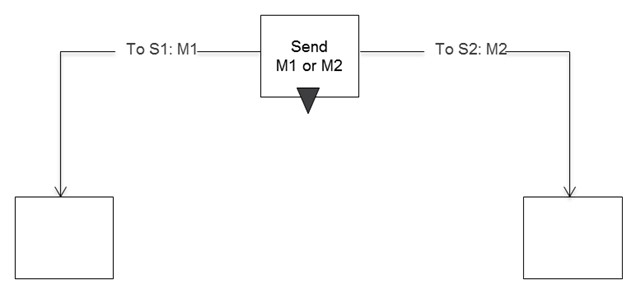
\includegraphics[width=0.7\linewidth]{Figures/Ontology/SubjectExecution/sendState}
	\caption[Example of alternative sending]{Example of alternative sending}
	\label{fig:sendstate}
\end{figure}

By specifying priorities, the order of sending can be influenced. For example, it can be determined that the message M1 to S1 has a higher priority than the message M2 to S2. Using this specification, the sending subject starts with sending message M1 to S1 and then tries only in case of failure to send message M2 to S2. In case of message M2 can also not be sent to the subject S2, the attempts to send start from the beginning.

The blocking of subjects when attempting to send can be monitored over time with the so-called timeout. The example in Figure \ref{fig:sendstatetimer} shows with 'Timeout: 24 h' an additional state transition which occurs when within 24 hours one of the two messages cannot be sent. If a value of zero is specified for the timeout, the process immediately follows the timeout path when the alternative message delivery fails.

\begin{figure*}[htbp]
	\centering
	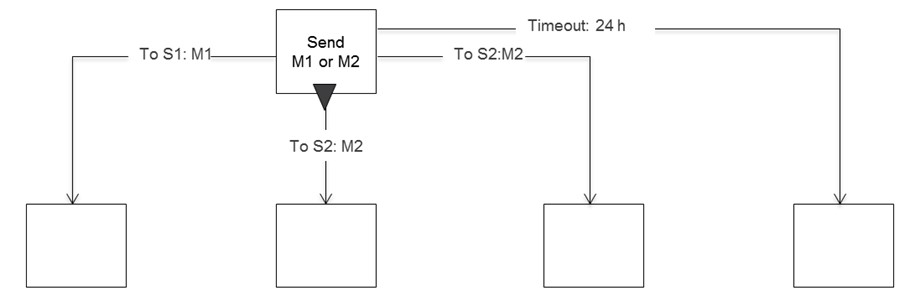
\includegraphics[width=0.7\linewidth]{Figures/Ontology/SubjectExecution/SendSTateTimer}
	\caption[Send using time monitoring]{Send using time monitoring}
	\label{fig:sendstatetimer}
\end{figure*}

\subsection{Receiving Messages}

Analogously to sending, the receiving procedure is divided into two phases, which run inversely to send.

The first step is to verify whether the expected message is ready for being picked up. In the case of synchronous messaging, it is checked whether the sending subject offers the message. In the asynchronous version, it is checked whether the message has already been stored in the input pool. If the expected message is accessible in either form, it is accepted, and in a second step, the corresponding state transition is performed. This leads to a takeover of the message parameters of the accepted message to local variables or business objects of the receiving subject. In case the expected message is not ready, the receiving subject is blocked until the message arrives and can be accepted.

In a certain state, a subject can expect alternatively multiple messages. In this case, it is checked whether any of these messages are available and can be accepted. The test sequence is arbitrary unless message priorities are defined. In this case, an available message with the highest priority is accepted. However, all other messages remain available (e.g., in the input pool) and can be accepted in other receive states.

Figure \ref{fig:receivestate} shows a receive state of the subject 'employee' which is waiting for the answer regarding a business trip request. The answer may be an approval or a rejection.

\begin{figure*}[htbp]
	\centering
	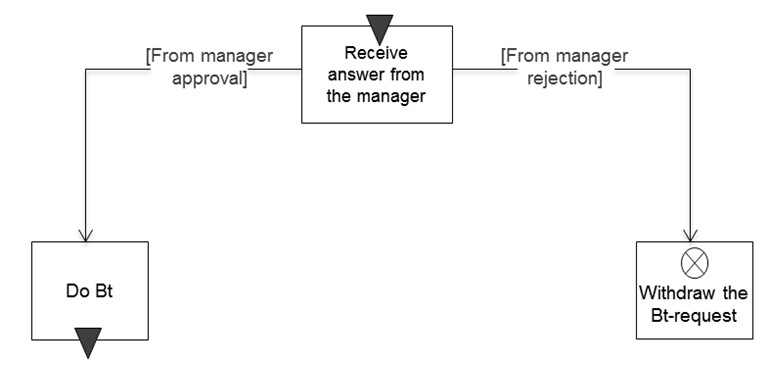
\includegraphics[width=0.7\linewidth]{Figures/Ontology/SubjectExecution/ReceiveState}
	\caption[Example of alternative receiving]{Example of alternative receiving}
	\label{fig:receivestate}
\end{figure*}

Just as with sending messages, also receiving messages can be monitored over time. If none of the expected messages are available and the receiving subject is therefore blocked, a time limit can be specified for blocking. After the specified time has elapsed, the subject will execute the transition as it is defined for the timeout period. The duration of the time limit may also be dynamic, in the sense that at the end of a process instance the process stakeholders assigned to the subject decide that the appropriate transition should be performed. We then speak of a manual timeout.

\begin{figure*}[htbp]
	\centering
	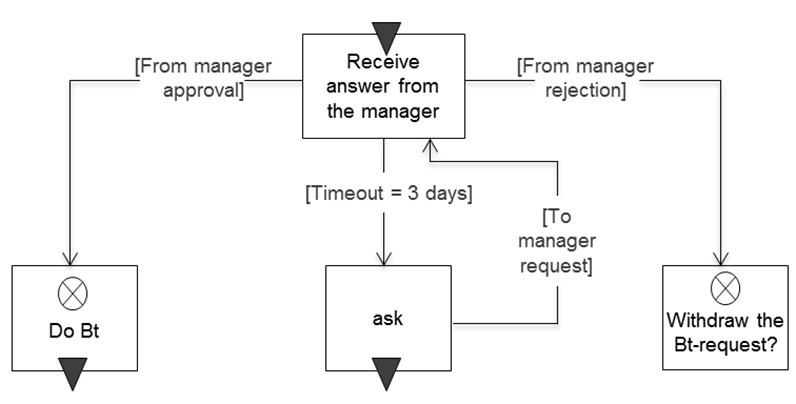
\includegraphics[width=0.7\linewidth]{Figures/Ontology/SubjectExecution/ReceiveStateTimer}
	\caption[Time monitoring for message reception]{Time monitoring for message reception}
	\label{fig:receivestatetimer}
\end{figure*}

Figure \ref{fig:receivestatetimer} shows that, after waiting three days for the manager's answer, the employee sends a corresponding request.

Instead of waiting for a message for a certain predetermined period of time, the waiting can be interrupted by a subject at all times. In this case, a reason for abortion can be appended to the keyword 'breakup'. In the example shown in Figure \ref{fig:receivestatebreak}, the receiving state is left due to the impatience of the subject.

\begin{figure*}[htbp]
	\centering
	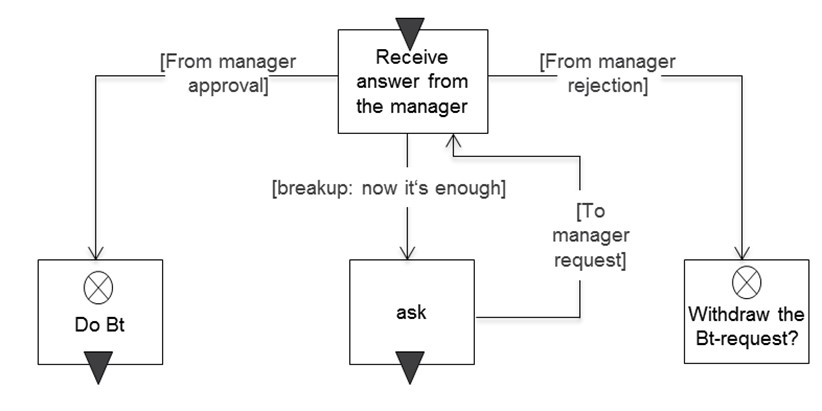
\includegraphics[width=0.7\linewidth]{Figures/Ontology/SubjectExecution/ReceiveStateBreak}
	\caption[Message reception with manual interrupt]{Message reception with manual interrupt}
	\label{fig:receivestatebreak}
\end{figure*}

\subsection{Standard Subject Behavior}

The possible sequences of a subject's actions in a process are termed subject behavior. States and state transitions describe what actions a subject performs and how they are interdependent. In addition to the communication for sending and receiving, a subject also performs so-called internal actions or functions.

States of a subject are therefore distinct: There are actions on the one hand, and communication states to interact with other subjects (receive and send) on the other. This results in three different types of states of a subject. Figure \ref{fig:behavior-symbole} shows the different types of states with the corresponding symbols.

\begin{figure*}[htbp]
	\centering
	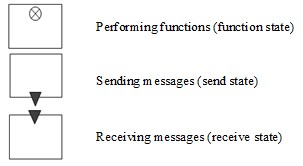
\includegraphics[width=0.5\linewidth]{Figures/Ontology/SubjectExecution/Behavior-Symbole}
	\caption[State types and coresponding symbols]{State types and coresponding symbols}
	\label{fig:behavior-symbole}
\end{figure*}

In S-BPM, work performers are equipped with elementary tasks to model their work procedures: sending and receiving messages and immediate accomplishment of a task (function state).

In case an action associated with a state (send, receive, do) is possible, it will be executed, and a state transition to the next state occurs. The transition is characterized through the result of the action of the state under consideration: For a send state, it is determined by the state transition to which subject what information is sent. For a receive state, it becomes evident in this way from what subject it receives which information. For a function state, the state transition describes the result of the action, e.g., that the change of a business object was successful or could not be executed.

The behavior of subjects is represented by modelers using Subject Behavior Diagrams (SBD). Figure \ref{fig:vollst-beispiel} shows the subject behavior diagram depicting the behavior of the subjects 'employee', 'manager', and 'travel office', including the associated states and state transitions. 

\begin{landscape}
	\begin{figure}[htbp]
		\centering
		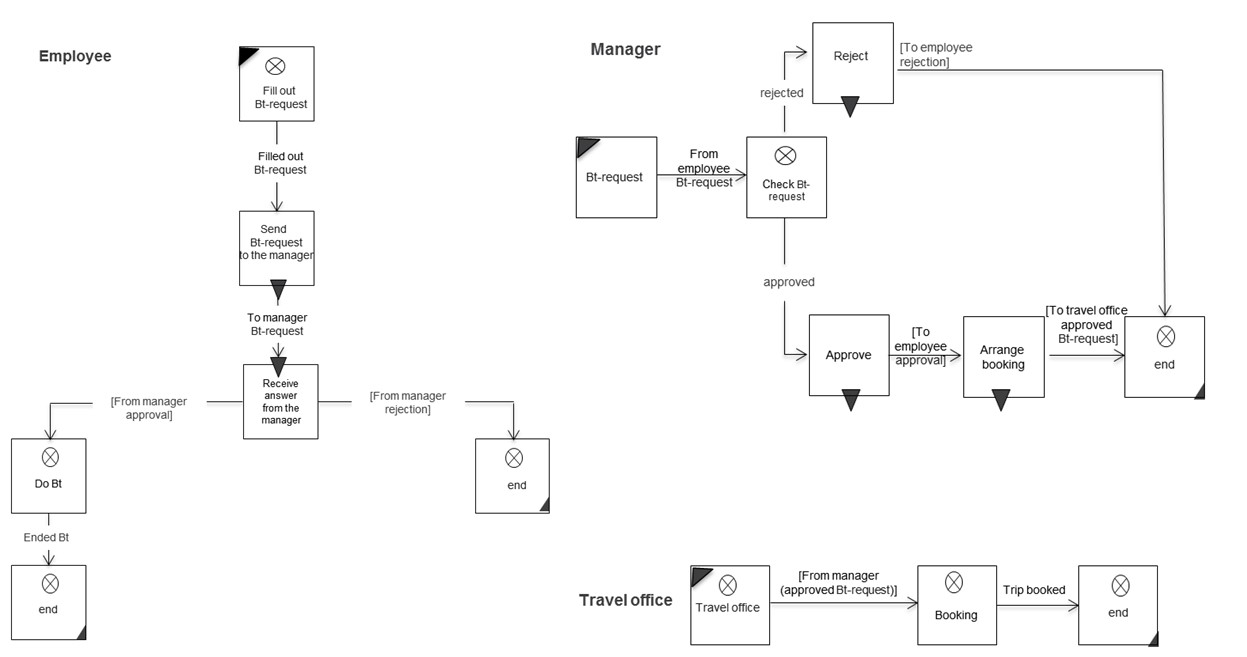
\includegraphics[width=0.9\linewidth]{Figures/Ontology/SubjectExecution/Vollst-Beispiel}
		\caption[Subject behavior diagram for the subjects 'employee', 'manager', and 'travel office']{Subject behavior diagram for the subjects 'employee', 'manager', and 'travel office'}
		\label{fig:vollst-beispiel}
	\end{figure}
\end{landscape}

\subsection{Extended Behavior}

To reduce description efforts some additional specification constructs have been added to PASS. These constructs are informally explained in the following sections. 

\subsubsection{Macros}

Quite often, a certain behavior pattern occurs repeatedly within a subject. This happens in particular when in various parts of the process identical actions need to be performed. If only the basic constructs are available to this respect, the same subject behavior needs to be described many times.

Instead, this behavior can be defined as a so-called behavior macro. Such a macro can be embedded at different positions of a subject behavior specification as often as required. Thus, variations in behavior can be consolidated, and the overall behavior can be significantly simplified.

The brief example of the business trip application is not an appropriate scenario to illustrate here the benefit of the use of macros. Instead, we use an example of order processing. Figure \ref{fig:macrobehavior} contains a macro for the behavior to process customer orders. After placing the 'order', the customer receives an order confirmation; once the 'delivery' occurs, the delivery status is updated.

As with the subject, the start and end states of a macro also need to be identified. For the start states, this is done similarly to the subjects by putting black triangles in the top left corner of the respective state box. In our example, 'order' and 'delivery' are the two correspondingly labeled states. In general, this means that a behavior can initiate a jump to different starting points within a macro.

The end of a macro is depicted by gray bars, which represent the successor states of the parent behavior. These are not known during the macro definition.

\begin{figure*}[htbp]
	\centering
	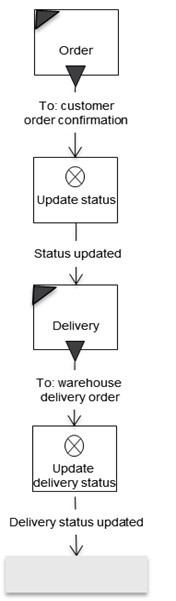
\includegraphics[width=0.2\linewidth]{Figures/Ontology/SubjectExecution/MacroBehavior}
	\caption[Behavior macro class 'request for approval']{Behavior macro class 'request for approval'}
	\label{fig:macrobehavior}
\end{figure*}

Figure \ref{fig:macrousage} shows a subject behavior in which the modeler uses the macro 'order processing' to model both a regular order (with purchase order), as well as a call order.

The icon for a macro is a small table, which can contain multiple columns in the first line for different start states of the macro. The valid start state for a specific case is indicated by the incoming edge of the state transition from the calling behavior. The middle row contains the macro name, while the third row again may contain several columns with possible output transitions, which end in states of the surrounding behavior.

The left branch of the behavioral description refers to regular customer orders. The embedded macro is labeled correspondingly and started with the status 'order', namely through linking the edge of the transition 'order accepted' with this start state. Accordingly, the macro is closed via the transition 'delivery status updated'.

The right embedding deals with call orders according to organizational frameworks and frame contracts. The macro starts therefore in the state 'delivery'. In this case, it also ends with the transition 'delivery status updated'.

\begin{figure}[htbp]
	\centering
	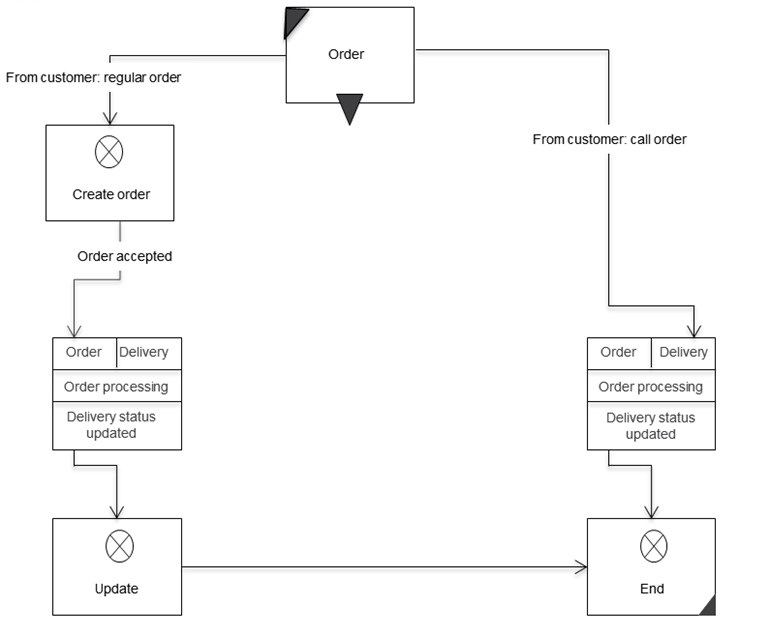
\includegraphics[width=0.6\linewidth]{Figures/Ontology/SubjectExecution/MacroUsage}
	\caption[Subject behavior for order processing with macro integration]{Subject behavior for order processing with macro integration}
	\label{fig:macrousage}
\end{figure}

Similar subject behavior can be combined into macros. When being specified, the environment is initially hidden, since it is not known at the time of modeling.

\subsubsection{Guards: Exception Handling and Extensions} 

\textbf{Exception Handling}---
Handling of an exception (also termed message guard, message control, message monitoring, message observer) is a behavioral description of a subject that becomes relevant when a specific, exceptional situation occurs while executing a subject behavior specification. It is activated when a corresponding message is received, and the subject is in a state in which it can respond to the exception handling. In such a case, the transition to exception handling has the highest priority and will be enforced.

Exception handling is characterized by the fact that it can occur in a process in many behavior states of subjects. The receipt of certain messages, e.g., to abort the process, always results in the same processing pattern. This pattern would have to be modeled for each state in which it is relevant. Exception handling causes high modeling effort and leads to complex process models since from each affected state a corresponding transition has to be specified. To prevent this situation, we introduce a concept similar to exception handling in programming languages or interrupt handling in operating systems.

To illustrate the compact description of exception handling, we use again the service management process with the subject 'service desk' introduced in section 5.6.5. This subject identifies a need for a business trip in the context of processing a customer order—an employee needs to visit the customer to provide a service locally. The subject 'service desk' passes on a service order to an employee. Hence, the employee issues a business trip request. In principle, the service order may be canceled at any stage during processing up to its completion. Consequently, this also applies to the business trip application and its subsequent activities.

Below, it is first shown how the behavior modeling looks without the concept of exception handling. The cancellation message must be passed on to all affected subjects to bring the process to a defined end. Figure \ref{fig:sid-exception} shows the communication structure diagram with the added cancellation messages to the involved subjects.

\begin{figure}[ph!]
	\centering
	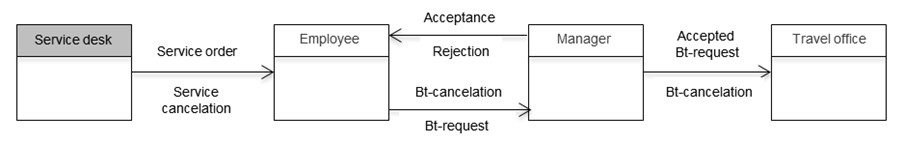
\includegraphics[width=0.7\linewidth]{Figures/Ontology/SubjectExecution/SID-Exception}
	\caption[Communication structure diagram (CSD) of the business trip application]{Communication structure diagram (CSD) of the business trip application}
	\label{fig:sid-exception}
\end{figure}

A cancellation message can be received by the employee either while filling out the application or while waiting for the approval or rejection message from the manager. Concerning the behavior of the subject 'employee', the state 'response received from manager' must also be enriched with the possible input message containing the cancellation and the associated consequences (see Figure \ref{fig:exceptionhandling}). The verification of whether filing the request is followed by a cancellation is modeled through a receive state with a timeout. In case the timeout is zero, there is no cancellation message in the input pool and the business trip request is sent to the manager. Otherwise, the manager is informed of the cancellation and the process terminates for the subject 'employee'.


\begin{figure}[htbp]
	\centering
	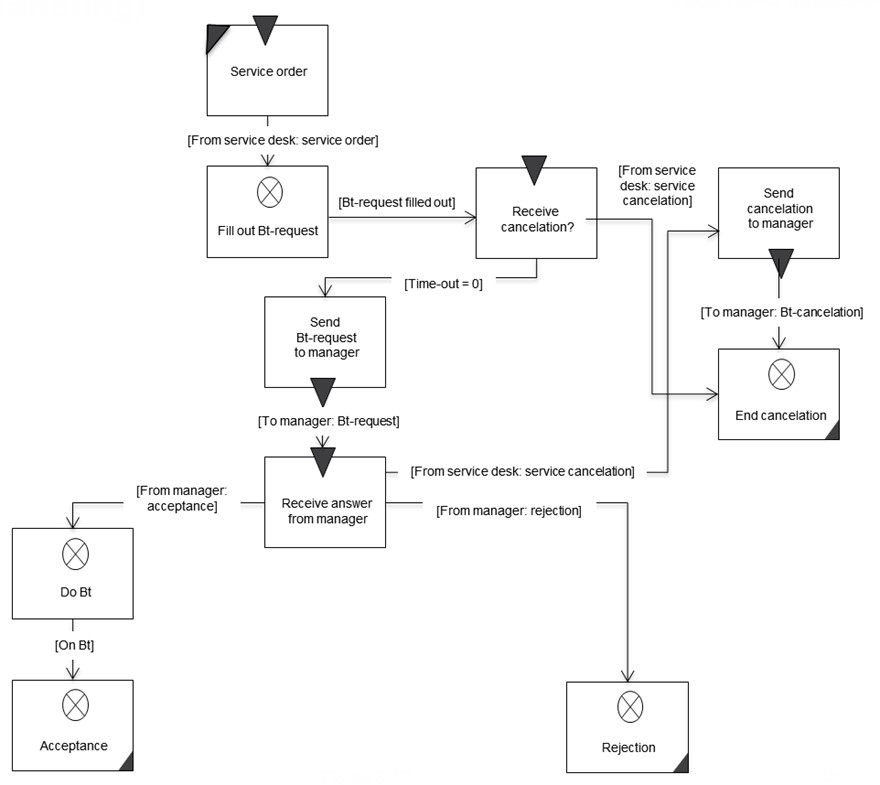
\includegraphics[width=0.7\linewidth]{Figures/Ontology/SubjectExecution/ExceptionHandling}
	\caption[Handling the cancelation message using existing constructs]{Handling the cancelation message using existing constructs}
	\label{fig:exceptionhandling}
\end{figure}

A corresponding adjustment of the behavior must be made for each subject which can receive a cancellation message, including the manager, the travel office, and the interface subject 'travel agent'.

This relatively simple example already shows that taking such exception messages into account can quickly make behavior descriptions confusing to understand. The concept of exception handling, therefore, should enable supplementing exceptions to the default behavior of subjects in a structured and compact form. 

\begin{figure}[htbp]
	\centering
	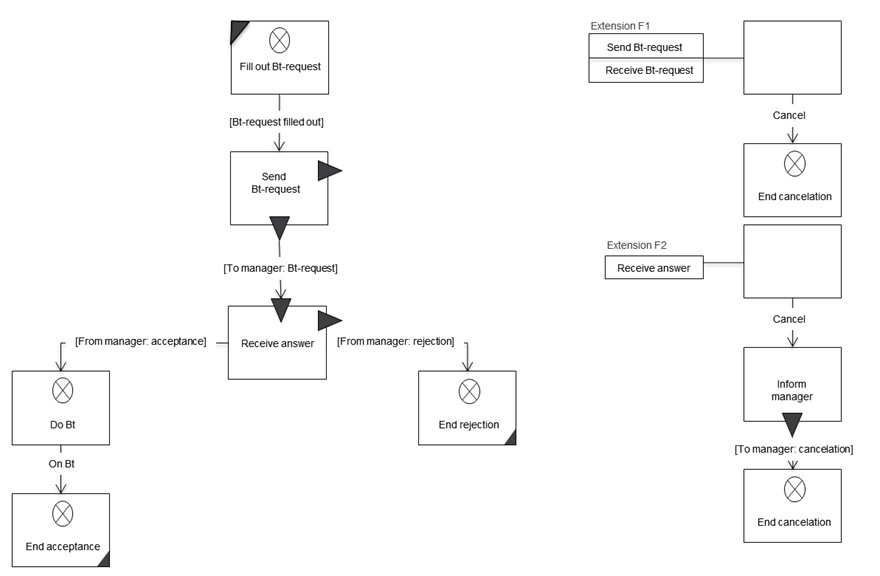
\includegraphics[width=0.7\linewidth]{Figures/Ontology/SubjectExecution/Extension}
	\caption[Behavior of subject 'employee' with exception handling]{Behavior of subject 'employee' with exception handling}
	\label{fig:extension}
\end{figure}

Instead of, as shown in Figure \ref{fig:exceptionhandling}, modeling receive states with a timeout zero and corresponding state transitions, the behavioral description is enriched with the exception handling 'service cancellation'. Its initial state is labeled with the states from which it is branched to, once the message 'service cancellation' is received. In the example, these are the states 'fill out Bt-request' and 'receive answer from manager'. Each of them is marked by a triangle on the right edge of the state symbol. The exception behavior leads to an exit of the subject after the message 'service cancellation' has been sent to the subject 'manager'.

A subject behavior does not necessarily have to be brought to an end by an exception handling; it can also return from there to the specified default behavior. Exception handling behavior in a subject may vary, depending on from which state or what type of message (cancellation, temporary stopping of the process, etc.) it is called. The initial state of exception handling can be a receive state or a function state.

Messages, like 'service cancellation', that lead to exception handling always have higher priority than other messages. This is how modelers express that specific messages are read in a preferred way. For instance, when the approval message from the manager is received in the input pool of the employee, and shortly thereafter the cancellation message, the latter is read first. This leads to the corresponding abort consequences.

Since now additional messages can be exchanged between subjects, it may be necessary to adjust the corresponding conditions for the input-pool structure. In particular, the input-pool conditions should allow storing an interrupt message in the input pool. To meet organizational dynamics, exception handling and extensions are required. They allow taking not only discrepancies but also new patterns of behavior, into account.

\textbf{Behavior Extensions}---
When exceptions occur, currently running operations are interrupted. This can lead to inconsistencies in the processing of business objects. For example, the completion of the business trip form is interrupted once a cancelation message is received, and the business trip application is only partially completed. Such consequences are considered acceptable, due to the urgency of cancelation messages. In less urgent cases, the modeler would like to extend the behavior of subjects in a similar way, however, without causing inconsistencies. This can be achieved by using a notation analogous to exception handling. Instead of denoting the corresponding diagram with 'exception', it is labeled with 'extension'.

Behavior extensions enrich a subject's behavior with behavior sequences that can be reached from several states equivocally.

For example, the employee may be able to decide on his own that the business trip is no longer required and withdraw his trip request. Figure \ref{fig:extension} shows that the employee can cancel a business trip request in the states 'send business trip request to manager' and 'receive answer from manager'. If the transition 'withdraw business trip request' is executed in the state 'send business trip request to manager', then the extension 'F1' is activated. It leads merely to canceling of the application. Since the manager has not yet received a request, he does not need to be informed.

In case the employee decides to withdraw the business trip request in the state 'receive answer from manager', then extension 'F2' is activated. Here, first the supervisor is informed, and then the business trip is canceled.

\begin{figure}[htbp]
	\centering
	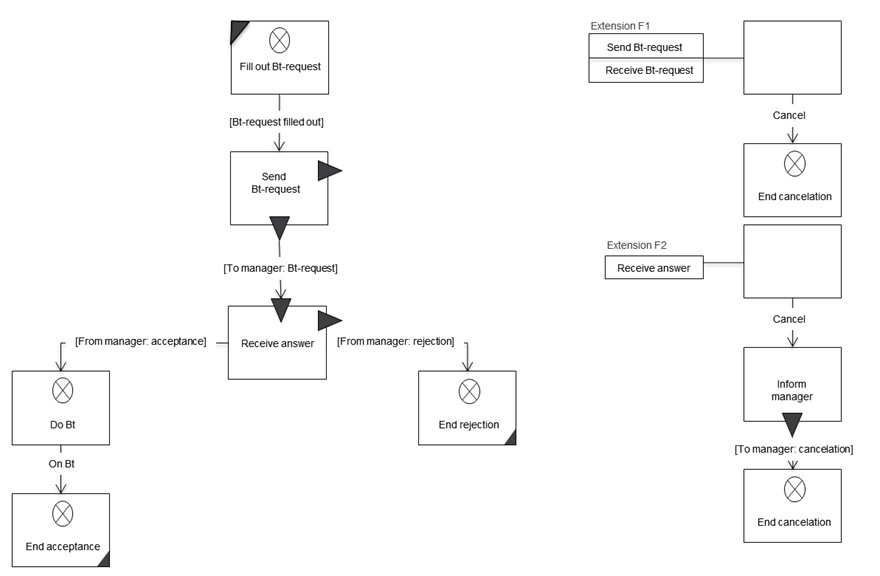
\includegraphics[width=0.7\linewidth]{Figures/Ontology/SubjectExecution/Extension}
	\caption[Subject behavior of employee with behavior extensions]{Subject behavior of employee with behavior extensions}
	\label{fig:extension}
\end{figure}

\subsubsection{Alternative Actions (Freedom of Choice)} 

So far, the behavior of subjects has been regarded as a distinct sequence of internal functions, send and receive activities. In many cases, however, the sequence of internal execution is not important.

Certain sequences of actions can be executed overlapping. We are talking about freedom of choice when accomplishing tasks. In this case, the modeler does not specify a strict sequence of activities. Rather, a subject (or concrete entity assigned to a subject) will organize to a particular extent its own behavior at runtime.

The freedom of choice with respect to behavior is described as a set of alternative clauses which outline several parallel paths. At the beginning and end of each alternative, switches are used: A switch set at the beginning means that this alternative path is mandatory to get started, a switch set at the end means that this alternative path must be completely traversed. This leads to the following constellations:

\begin{itemize}
	\item Beginning is set/end is set: Alternative needs to be processed to the end.
	\item Beginning is set/end is open: Alternative must be started but does not need to be finished. 
	\item Beginning is open/end is set: Alternative may be processed, but if so must be completed.
	\item Beginning is open/end is open: Alternative may be processed but does not have to be completed.
\end{itemize}

The execution of an alternative clause is considered complete when all alternative sequences, which were begun and had to be completed, have been entirely processed and have reached the end operator of the alternative clause.

Transitions between the alternative paths of an alternative clause are not allowed. An alternate sequence starts in its start point and ends entirely within its endpoint.

Figure \ref{fig:alternative} shows an example for modeling alternative clauses. After receiving an order from the customer, three alternative behavioral sequences can be started, whereby the leftmost sequence, with the internal function 'update order' and sending the message 'deliver order' to the subject 'warehouse', must be started in any case. This is determined by the 'X' in the symbol for the start of the alternative sequences (the gray bar is the starting point for alternatives). This sequence must be processed through to the end of the alternative because it is also marked in the end symbol of this alternative with an 'X' (gray bar as the endpoint of the alternative).

\begin{figure}[htbp]
	\centering
	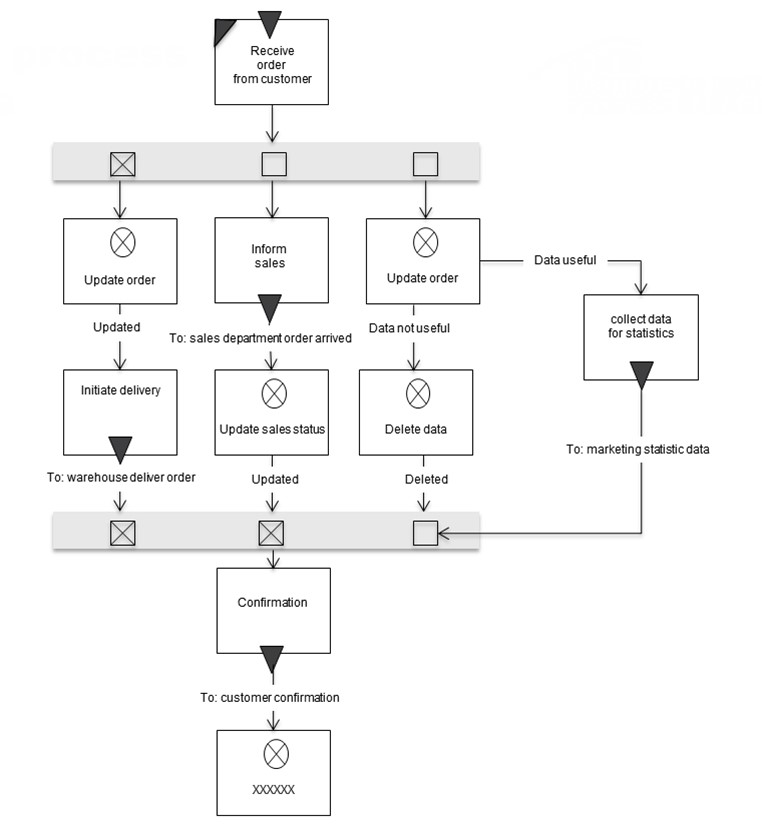
\includegraphics[width=0.7\linewidth]{Figures/Ontology/SubjectExecution/ALternative}
	\caption[Example of Process Alternatives]{Example of Process Alternatives}
	\label{fig:alternative}
\end{figure}

The other two sequences may, but do not have to be, started. However, in case the middle sequence is started, i.e., the message 'order arrived' is sent to the sales department, it must be processed to the end. This is defined by an appropriate marking in the end symbol of the alternatives ('X' in the lower gray bar as the endpoint of the alternatives). The rightmost path can be started but does not need to be completed.

The individual actions in the alternative paths of an alternative clause may be arbitrarily executed in parallel and overlapping, or in other words: A step can be executed in an alternative sequence, and then be followed by an action in any other sequence. This gives the performer of a subject the appropriate freedom of choice while executing his actions.

In the example, the order can thus first be updated, and then the message 'order arrived' sent to sales. Now, either the message 'deliver order' can be sent to the warehouse or one of the internal functions, 'update sales status' or 'collect data for statistics', can be executed.

The left alternative must be executed completely, and the middle alternative must also have been completed, if the first action ('inform sales' in the example) is executed. Only the left alternative can be processed because the middle one was never started. Alternatively, the sequence in the middle may have already reached its endpoint, while the left is not yet complete. In this case, the process waits until the left one has reached its endpoint. Only then will the state 'confirmation' be reached in the alternative clause. The right branch neither needs to be started, nor to be completed. It is therefore irrelevant for the completion of the alternative construct.

The leeway for freedom of choice with regards to actions and decisions associated with work activities can be represented through modeling the various alternatives—situations can thus be modeled according to actual regularities and preferences.

\section{Ontology of Subject Behavior Description}

Each subject has a base behavior (see property 202 in \ref{fig:20190104-simple-elements-and-modellelement}) and may have additional subject behaviors (see class \texttt{SubjectBehavior} in \ref{fig:20190104-simple-elements-and-modellelement}) for macros and guards. All these behaviors are subclasses of the class \texttt{SubjectBehavior}. The details of these behaviors are defined as state transition diagrams (PASS behavior diagrams). These behavior diagrams are represented in the ontology with the class \texttt{BehaviorDescribingComponent} (see figure \ref{fig:20190104-simple-elements-and-modellelement}). The behavior diagrams have the relation \texttt{belongsTo} to the class \texttt{SubjectBehavior}. The other classes are needed for \texttt{embeddingsubjects} into the subject interaction diagram (SID) of a PASS specification (see chapter \ref{OWL-DescriptionSID}).

\begin{figure}[htbp]
	\centering
	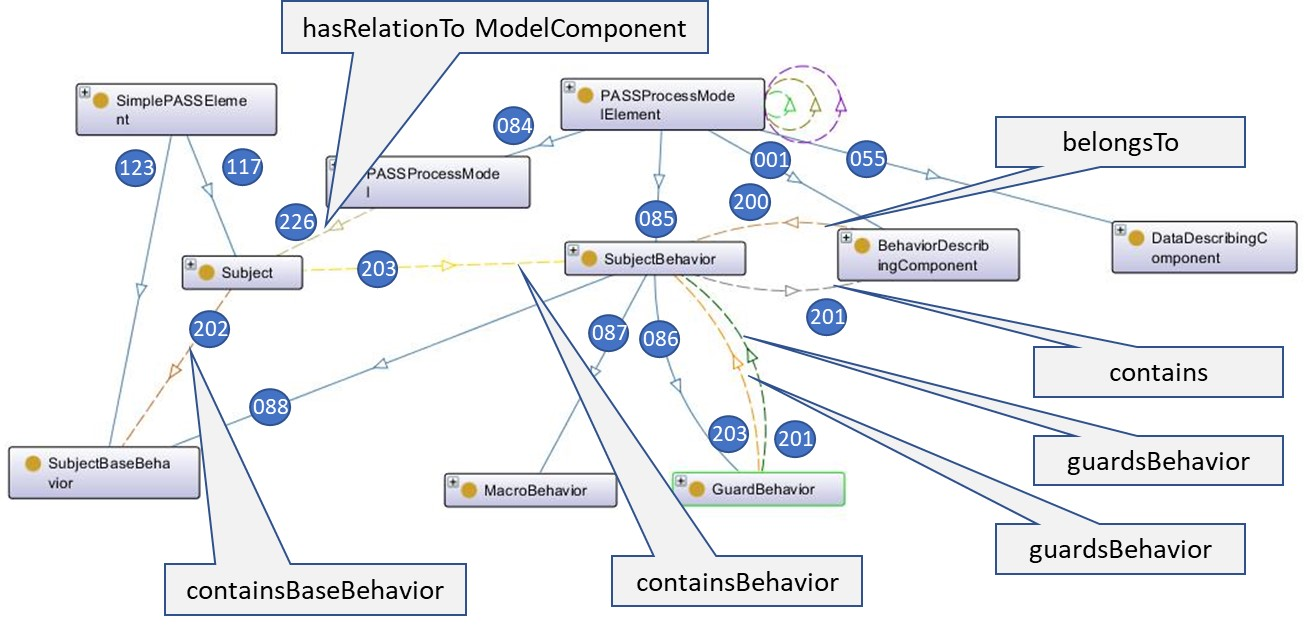
\includegraphics[width=0.9\linewidth]{Figures/Ontology/SubjectExecution/20190104-SImple-Elements-and-Modellelement}
	\caption[Structure of Subject Behavior Specification]{Structure of Subject Behavior Specification}
	\label{fig:20190104-simple-elements-and-modellelement}
\end{figure}

\subsection{Behavior Describing Component}

The following figure shows the details of the class \texttt{BehaviorDescribingComponent}. This class has the subclasses State, Transition and \texttt{TranssitionCondition} (see figure \ref{fig:20190104-behavior-describing-component}). The subclasses of the state represent the various types of states (class relations 025, 014 und 024 in \ref{fig:20190104-behavior-describing-component}). The standard states \texttt{DoSTates}, \texttt{SendState} and \texttt{ReceiveState} are subclasses of the class \texttt{StandardPASSState} (class relations 114, 115 und 116 in \ref{fig:20190104-behavior-describing-component}). The subclass relations 104 and 020 allow that there exist a start state (class \texttt{InitialStatOfBehavior} in \ref{fig:20190104-behavior-describing-component}) and none or several end states (see subclass relation 020 in figure\ref{fig:20190104-behavior-describing-component}) The fact that there must be at least one start state and none or several end states is defined by so called axioms which are not shown in figure \ref{fig:20190104-behavior-describing-component}.

\begin{figure}[htbp]
	\centering
	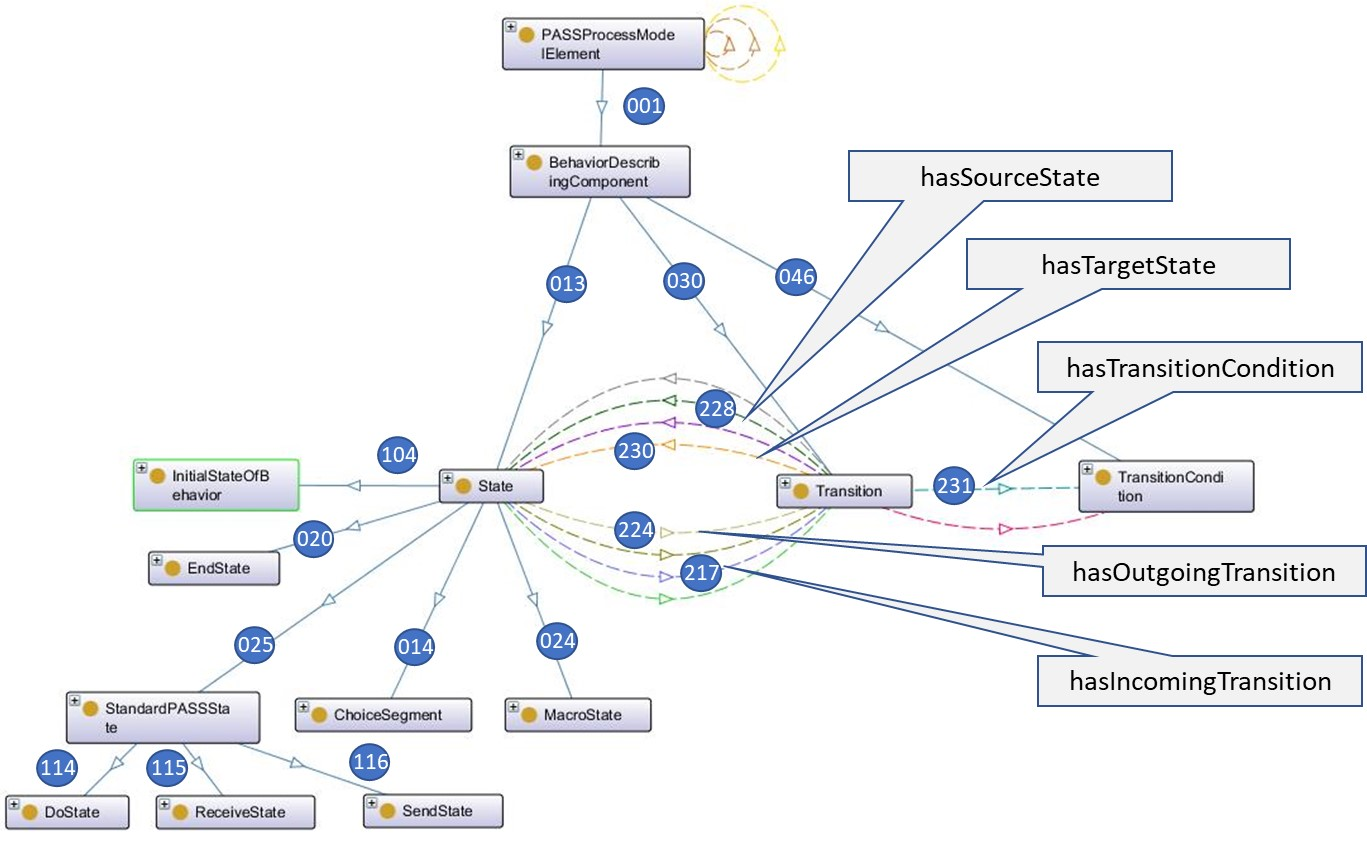
\includegraphics[width=1.0\linewidth]{Figures/Ontology/SubjectExecution/20190104-Behavior-describing-component}
	\caption[Subject Behavior describingComponent]{Subject Behavior describingComponent}
	\label{fig:20190104-behavior-describing-component}
\end{figure}

States can be starting and/or endpoints of transitions (see properties 228 and 230 in figure \ref{fig:20190104-behavior-describing-component}). This means a state may have outgoing and/or incoming transitions (see properties 224 and 217 in figure \ref{fig:20190104-behavior-describing-component}). Each transition is controlled by a transition condition which must be true before a behavior follows a transition from the source state to the target state.

\subsubsection{States}

As shown in figure \ref{fig:20190109-states} the class state has a subclass \texttt{StandardPASSState} (subclass relation 025) which have the subclasses \texttt{ReceiveState}, \texttt{SendState} and \texttt{DoState}(subclass relations 027, 026, 025). A state can be a start state (subclass \texttt{InitialStateOfBehavior} subclass relation 022). Besides these standard states there are macro states (subclass 024). Macro states contain a reference (subclass 029) to the corresponding macro (Property 201).

\begin{figure}[htbp]
	\centering
	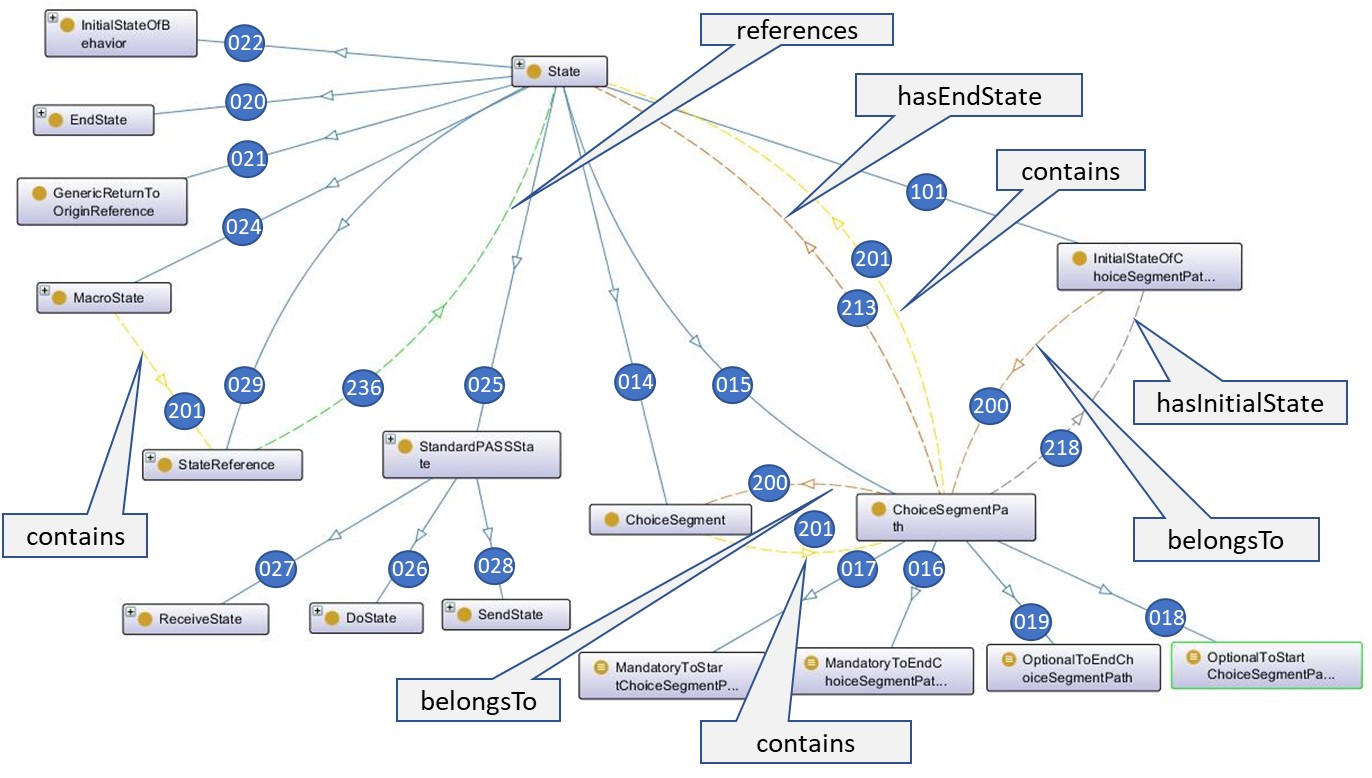
\includegraphics[width=1.0\linewidth]{Figures/Ontology/SubjectExecution/20190109-States}
	\caption[Details of States]{Details of States}
	\label{fig:20190109-states}
\end{figure}

More complex states are choice segments (subclass relation 014). A choice segment contains choice segment paths (subclass 015 and property 200). Each choice segment path can be of one of four types. If a segment path is started than it must be finished or not or a segment path must be started and must be finished or not (subclass relations 16, 17, 18 and 19).

\subsubsection{Transitions}

Transitions connect the source state with the target state (see figure \ref{fig:20190104-behavior-describing-component}). A transition can be executed if the transition condition is valid. This means the state of a behavior changes from the current state which is the source state to the target state. In PASS there are two basic types of transitions, \texttt{DoTransitions} and \texttt{CommunicationTranstions} (subclasses 34 and 31 in figure \ref{fig:20190105-transitions}). The class \texttt{CommunicationTransition} is divided into the subclasses \texttt{ReceiveTransition} and \texttt{SendTransition} (subclasses 32 and 33 in figure \ref{fig:20190105-transitions}). Each transition has depending from its type a corresponding transition condition (property 231 in figure  \ref{fig:20190105-transitions}) which defines a data condition which must be valid in in order to execute a transition.

\begin{figure}[htbp]
	\centering
	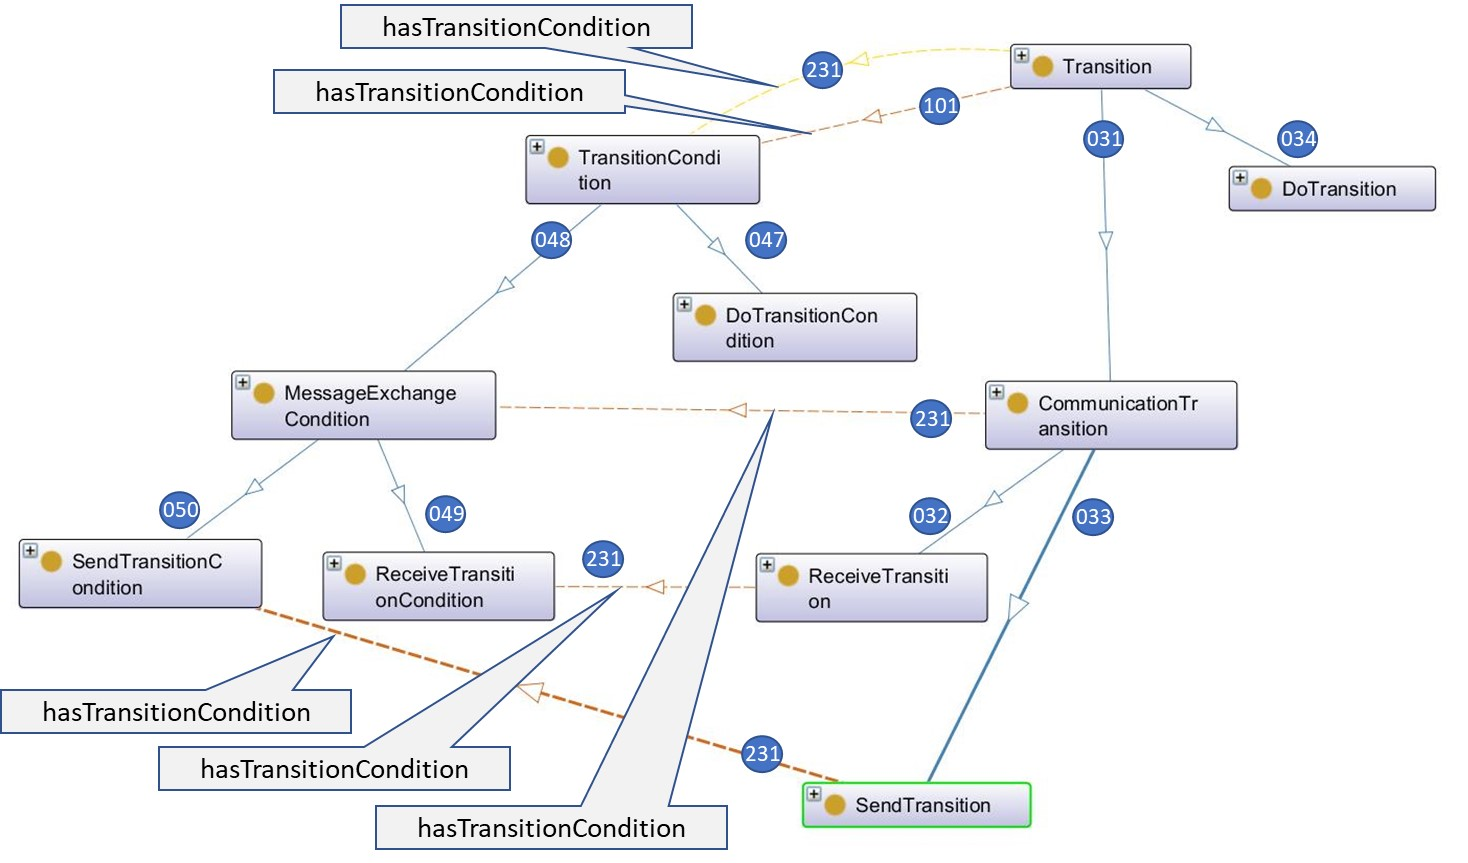
\includegraphics[width=1.0\linewidth]{Figures/Ontology/SubjectExecution/20190105-Transitions}
	\caption[Details of transitions]{Details of transitions}
	\label{fig:20190105-transitions}
\end{figure}

\section{ASM Definition of Subject Execution}

\setminted{fontsize=\small}
\setmintedinline{fontsize=\normalsize,breaklines}

% NOTE: DRAFT WOLSKIA

This section provides a reduced overview of the ASM semantics given in Appendix~\ref{CoreASM-Reference-Implementation}.

The goal of this section is to provide a minimal set of reduced rules to establish a foundation to understand the ASM semantics,
leaving out certain features and implementation details.
It is therefore just an informal introduction to the topic.

Please note the conceptual differences between the interpreter semantics and the owl structure, presented in \ref{CoreASM-Reference-Implementation-Differences-OWL-Model}.
Most importantly, the interpreter semantics for interaction support only "IP strategy blocking".

simplifications for this chapter:
\begin{itemize}
	\item no Observer support => no execution state, no state priorities => Cancel not required
	\item limited scope to InternalAction, Send, Receive, CallMacro, ModalSplit/ModalJoin, End => no VarMan, Cancel, SelectAgents, Tau
	\item discuss: proper-termination and CloseIP/OpenIP are motivated from interaction soundness. include? mention? hard-exclude (remove references from code)?
	\item no KillBehavior (although recursive macros and reservation messages). therefore this will not be sound - but a bit less complicated
\end{itemize}

\subsection{Foundation}

The interpreter uses asynchronous multi-agent Turbo ASMs.
It supports the concurrent execution of multiple process models and multiple instances of each process model.
Each instance has a unique \textit{ProcessInstanceID} (short: \asminline{PI}) assigned.
Within a process instance multiple instances of a subject can occur (MultiSubject concept).
Each subject instance has an agent assigned, to distinguish the subject instances.
This agent is identified by it name.
We therefore identify a subject instance by the tuple (Process~Model~ID, Process~Instance~ID, Subject~ID, Agent~Name).
This tuple is called \textit{Channel} (short: \asminline{ch}), as it used in the mobility of channels concept in order to support distributed communication patterns.

In the interpreter, each subject instance has an ASM Agent assigned, that keeps track of its current state,
where we mean state in the sense of which subject data is present, the content of the inputpool queues and also the active SBD states.
This state is stored in ASM functions and assigned to the \textit{Channel}.

\begin{listing}[H]
	\begin{minted}{lexer.py:CoreASMLexer -x}
		// ASM Agent -> Channel
		function channelFor : Agents -> LIST
		
		derived processIDFor(a)       = processIDOf(channelFor(a))
		derived processInstanceFor(a) = processInstanceOf(channelFor(a))
		derived subjectIDFor(a)       = subjectIDOf(channelFor(a))
		derived agentFor(a)           = agentOf(channelFor(a))
		
		derived processIDOf(ch)       = nth(ch, 1)
		derived processInstanceOf(ch) = nth(ch, 2)
		derived subjectIDOf(ch)       = nth(ch, 3)
		derived agentOf(ch)           = nth(ch, 4)
	\end{minted}
	\caption{Channel definitions}
	\label{lst:shortasm:channelFor}
\end{listing}

In the function \asminline{channelFor} the assignment from the ASM Agents to their \textit{Channels} is stored. The derived functions are used to lookup certain tuple elements of the channel.

% NOTE: StartProcess and StartASMAgent left out intentionally

% Subject Data

Analogous to programming languages we call Subject Data \textit{Variables}.
Their scope is either bound to a Subject or a Macro Instance and can only be
accessed by the Subject. Variables are identified by their name and have an
explicit data type and a value.

Variables are stored in the \asminline{variable} function which maps from
the Subject's Channel, the scoped Macro Instance~ID and the Variable's name to
a pair of the data type and value. For Variables that are not scoped to a Macro
Instance, and are therefore accessible for any state in any Macro Instance of
the Subject, the unused Macro Instance~ID~0 is used.

The function \asminline{variableDefined} is used to keep track of Variables
that are in use, so that their content can be reset upon the termination of a
Macro Instance or the Subject, respectively.

\begin{listing}[H]
	\begin{minted}{lexer.py:CoreASMLexer -x}
		// Channel * macroInstanceNumber * varname -> [vartype, content]
		function variable : LIST * NUMBER * STRING -> LIST
		
		// Channel -> Set[(macroInstanceNumber, varname)]
		function variableDefined : LIST -> SET
	\end{minted}
	\caption{variable}
	\label{lst:shortasm:variable}
\end{listing}

\subsection{Interaction Definitions}\label{sec:InteractionDefinitions}

We implement the interaction between Subjects as asynchronous Message exchange.
Messages are placed into the Inputpool of the receiver where they are then retrieved from when the receiver is in a Receive state.

\subsubsection{Messages}\label{sec:messages}

The message content consists of the actual payload and its data type. As this
reference implementation is intended only for an abstract process execution we abstract
the payload / business objects to be just a text given as string.

For the communication with MultiSubjects, i.e. sending the same Message to
multiple Agents of one Subject, we use an \textit{all-or-none} strategy. This
is accomplished by separating the sending of a Message into two phases: first
a reservation Message is placed at each receiver into the Inputpool.
Only after all reservations could be placed they are then replaced with the
actual Message.

\subsubsection{Inputpool}\label{sec:Inputpool}

The Inputpool is structured into multiple FIFO queues per Subject~ID of the sender, the Messagetype and the CorrelationID.

The Inputpool can be limited to allow a maximum number of Messages and
reservations per sender Subject~ID and Messagetype; in case the Inputpool Limit is
reached no additional reservation can be placed. To support the proper
termination of a Subject a specific queue (and also the complete Inputpool)
can be closed, in which case no additional reservation can be placed into it,
too.

\begin{listing}[H]
	\begin{minted}{lexer.py:CoreASMLexer -x}
		// receiverChannel * senderSubjID * messageType * correlationID -> [msg1, msg2, ...]
		function inputPool : LIST * STRING * STRING * NUMBER -> LIST
		
		/* store all locations where an inputPool was defined for to allow IPEmpty and receiving from "?" */
		// receiverChannel -> {[senderSubjID, messageType, correlationID], ..}
		function inputPoolDefined : LIST -> SET
		
		// receiverChannel * senderSubjID * messageType * correlationID
		function inputPoolClosed : LIST * STRING * STRING * NUMBER -> BOOLEAN
	\end{minted}
	\caption{inputPool}
	\label{lst:shortasm:inputPool}
\end{listing}

The queues of the Inputpool are stored in the \asminline{inputPool} function.
The function \asminline{inputPoolDefined} is used to keep track of the
locations of the queues that are in use, so that their content can be checked
upon termination. The function \asminline{inputPoolClosed} is used to store
whether a queue is closed. The special location
\asminline{inputPoolClosed(ch, undef, undef, undef)} is used to
store whether the complete Inputpool is closed.

We define the function \asminline{derived availableMessages(receiverChannel, senderSubjectID, msgType, ipCorrelationID)} to return the Messages from the location \asminline{inputPool(receiverChannel, senderSubjectID, msgType, ipCorrelationID)} that can be received, i.e. that it filters out reservations and reduces Messages from the same sender to only the oldest one.

\subsection{Subject Behavior}

As depicted in figure~\ref{fig:MainSBPM components}, a Subject Behavior consists at least of one \textit{Main Macro} and might have an arbitrary number of minor Macros, called \textit{Additional Macros}.

\begin{listing}[H]
	\begin{minted}{lexer.py:CoreASMLexer -x}
		rule SubjectBehavior =
		MacroBehavior(1)
	\end{minted}
	\caption{SubjectBehavior}
	\label{lst:shortasm:SubjectBehavior}
\end{listing}

% Macro Behavior

% NOTE: extemely shortened: no execution state => no remainingStates

The \asminline{MacroBehavior} rule controls the evaluation of all active
states for the given Macro Instance~ID~\asminline{MI}.

\begin{listing}[H]
	\begin{minted}{lexer.py:CoreASMLexer -x}
		rule MacroBehavior(MI) =
		let ch = channelFor(self) in
		choose stateNumber in activeStates(ch, MI) do
		Behavior(MI, stateNumber)
	\end{minted}
	\caption{MacroBehavior}
	\label{lst:shortasm:MacroBehavior}
\end{listing}

From that list a state \asminline{stateNumber} is chosen to be evaluated with the \asminline{Behavior} rule.

% State

The evaluation of a state is structured into three main phases: initialization,
the state function and an optional transition behavior.

The state function is responsible for the selection of an outgoing transition and
has to supervise the Timeout. It also has to enable and disable its outgoing
transitions, meaning that transitions can be available depending on some dynamic state,
for example whether a certain Message is present in the Inputpool.
Usually the outgoing transition will be selected by the environment, however with
auto-transitions it is possible that such an transition is automatically selected as soon
as it becomes enabled and as long as there are no other transitions to select from.

\begin{listing}[H]
	\begin{minted}{lexer.py:CoreASMLexer -x}
		rule Behavior(MI, currentStateNumber) =
		let s = currentStateNumber,
		ch = channelFor(self) in
		if (initializedState(ch, MI, s) != true) then
		StartState(MI, s)
		else if (abortState(MI, s) = true) then
		AbortState(MI, s)
		else if (completed(ch, MI, s) != true) then
		Perform(MI, s)
		else if (initializedSelectedTransition(ch, MI, s) != true) then
		StartSelectedTransition(MI, s)
		else
		let t = selectedTransition(ch, MI, s) in
		if (transitionCompleted(ch, MI, t) != true) then
		PerformTransition(MI, s, t)
		else
		Proceed(MI, s, targetStateNumber(processIDFor(self), t))
	\end{minted}
	\caption{Behavior}
	\label{lst:shortasm:Behavior}
\end{listing}

In the beginning the \asminline{Behavior} rule initializes the state with the
\asminline{StartState} rule, which will set \asminline{initializedState} to
\asminline{true}. If the function should not be aborted the \asminline{Perform}
rule calls the state behavior of the underlying function until it is
\asminline{completed}.
In the next phase the selected transition will be initialized by the
\asminline{StartSelectedTransition} rule and the transition behavior will be performed with
the \asminline{PerformTransition} rule until it is completed as well. As last step
the \asminline{Proceed} rule removes the current state and adds the selected
transition's target state.

%---

The environment has full read access to all functions of this semantics and knows
therefore each running Subject, their Macro Instances and their active states.

To define a homogeneous interface between the Function semantics and the environment we
define the function \asminline{wantInput} to be written by an Function when it
requires an external input, for example if an outgoing transition has to be chosen.

\begin{listing}[H]
	\begin{minted}{lexer.py:CoreASMLexer -x}
		// Channel * MacroInstanceNumber * StateNumber -> Set[String]
		function wantInput : LIST * NUMBER * NUMBER -> SET
	\end{minted}
	\caption{wantInput}
	\label{lst:shortasm:wantInput}
\end{listing}

This function is read by our console application for all active states
to present the user a list of possible decisions that can be made.

The environment then writes its external input in a corresponding function, for
example for a transition decision into the \asminline{selectedTransition} function, and
clears the \asminline{wantInput} function of that state.

The \asminline{SelectTransition} rule adds the \asminline{"TransitionDecision"}
requirement into the \asminline{wantInput} function.

\begin{listing}[H]
	\begin{minted}{lexer.py:CoreASMLexer -x}
		rule SelectTransition(MI, currentStateNumber) =
		let ch = channelFor(self),
		s = currentStateNumber in
		if (|outgoingEnabledTransitions(ch, MI, s)| = 0) then
		skip // BLOCKED: none to select
		else if (not(contains(wantInput(ch, MI, s),
		"TransitionDecision"))) then
		add "TransitionDecision" to wantInput(ch, MI, s)
		else
		skip // waiting for selectedTransition
	\end{minted}
	\caption{SelectTransition}
	\label{lst:shortasm:SelectTransition}
\end{listing}


If the \asminline{wantInput} function already contains the
\asminline{"TransitionDecision"} requirement nothing needs to be done and another
state can be evaluated by the \asminline{MacroBehavior} rule.
The same applies if there are no outgoing transitions enabled.
Otherwise the requirement is added to the \asminline{wantInput} function.

\subsection{Internal Action}

The \emph{Internal Action} is used to model DoStates, Subject-internal activities and decisions.
It is labeled with a textual description of the activity that the Agent should perform.
The outgoing transitions are labeled with a textual description of the possible execution results.
Since the activity is performed outside of the interpreter all outgoing transitions are enabled from the beginning on and no transition rule has to be defined.
Therefore the state function only consists of the timeout check and transition selection.

\begin{listing}[H]
	\begin{minted}{lexer.py:CoreASMLexer -x}
		rule StartInternalAction(MI, currentStateNumber) = {
			StartTimeout(MI, currentStateNumber)
			
			EnableAllTransitions(MI, currentStateNumber)
		}
	\end{minted}
	\caption{StartInternalAction}
	\label{lst:shortasm:StartInternalAction}
\end{listing}

The initialization of the InternalAction starts the Timeout and enables all
outgoing transitions.

\begin{listing}[H]
	\begin{minted}{lexer.py:CoreASMLexer -x}
		rule PerformInternalAction(MI, currentStateNumber) =
		let ch = channelFor(self),
		s = currentStateNumber in
		if (shouldTimeout(ch, MI, s) = true) then {
			SetCompleted(MI, s)
			ActivateTimeout(MI, s)
		}
		else if (selectedTransition(ch, MI, s) != undef) then
		SetCompleted(MI, s)
		else
		SelectTransition(MI, s)
	\end{minted}
	\caption{PerformInternalAction}
	\label{lst:shortasm:PerformInternalAction}
\end{listing}


The state function checks if a Timeout should be activated; otherwise the
\asminline{SelectTransition} rule is called until the \asminline{selectedTransition} function has
been set.

\subsection{Send Function}

The Send Function sends a Message. Disregarding the optional Timeout and Cancel
transitions it must have exactly one outgoing transition which has to have parameters that
define at least the Messagetype and the receiver's Subject~ID.

We use an \textit{all-or-none} strategy to send Messages to MultiSubjects,
which means that the actual Message is only send when all receivers are able
to store it in their Inputpool. Therefore the Send Function is structured into
two phases: in the first phase, realized as state function, reservation Messages
are placed and in the second phase, realized as transition function, these reservations
are replaced with the actual Message.

To place a reservation in a receiver's Inputpool there must be space available
in the corresponding queue and the receiver must not be
\textit{non-proper} terminated.

\begin{listing}[H]
	\begin{minted}{lexer.py:CoreASMLexer -x}
		// Channel * MacroInstanceNumber * StateNumber -> Set[Messages]
		function receivedMessages : LIST * NUMBER * NUMBER -> SET
		
		// Channel * MacroInstanceNumber * StateNumber -> Set[Channel]
		function receivers : LIST * NUMBER * NUMBER -> SET
		
		// Channel * MacroInstanceNumber * StateNumber
		function messageContent               : LIST * NUMBER * NUMBER -> LIST
		function messageCorrelationID         : LIST * NUMBER * NUMBER -> NUMBER
		function messageReceiverCorrelationID : LIST * NUMBER * NUMBER -> NUMBER
		
		// Channel * MacroInstanceNumber * StateNumber -> Set[Channel]
		function reservationsDone : LIST * NUMBER * NUMBER -> SET
		
		function nextCorrelationID : -> NUMBER
		function nextCorrelationIDUsedBy : NUMBER -> Agents
	\end{minted}
	\caption{receivedMessages}
	\label{lst:shortasm:receivedMessages}
\end{listing}

The Send Function stores the message content it has to send in the
\asminline{messageContent} function. The \asminline{receivers} function is
used to store the required receivers. When a reservation message has been
placed at a receiver its Channel is added to the \asminline{reservationsDone}
function.

The global function \asminline{nextCorrelationID} is used to increment
CorrelationIDs. To ensure the uniqueness of a CorrelationID the
\asminline{nextCorrelationIDUsedBy} function is used to store the ASM agent
that used the given CorrelationIDs.

\begin{listing}[H]
	\begin{minted}{lexer.py:CoreASMLexer -x}
		rule StartSend(MI, currentStateNumber) =
		let ch = channelFor(self),
		pID = processIDFor(self),
		s = currentStateNumber in
		// there must be exactly one transition
		let  t = first_outgoingNormalTransition(pID, s) in {
			receivers(ch, MI, s) := undef
			reservationsDone(ch, MI, s) := {}
			let mcVName = messageContentVar(pID, t) in
			messageContent(ch, MI, s) := loadVar(MI, mcVName)
			
			// generate new CorrelationID now, it will be stored
			// in a Variable once the message(s) are send
			let cIDVName = messageNewCorrelationVar(pID, t) in
			if (cIDVName != undef and cIDVName != "") then {
				messageCorrelationID(ch, MI, s) := nextCorrelationID
				nextCorrelationID := nextCorrelationID + 1
				// ensure no other agent uses this same correlationID
				nextCorrelationIDUsedBy(nextCorrelationID) := self
			}
			else
			messageCorrelationID(ch, MI, s) := 0
			
			// load receiver IP CorrelationID now, to avoid
			// influences of any changes of that variable
			let cIDVName = messageWithCorrelationVar(pID, t) in
			let cID = loadCorrelationID(MI, cIDVName) in
			messageReceiverCorrelationID(ch, MI, s) := cID
		}
	\end{minted}
	\caption{StartSend}
	\label{lst:shortasm:StartSend}
\end{listing}

The initialization of the Send Function resets / initializes the \asminline{receivers} and
\asminline{reservationsDone} functions.
If the communication transition has a \asminline{messageContentVar} parameter given the
content of that Variable is loaded and stored in the \asminline{messageContent}
function. If it has a \asminline{messageNewCorrelationVar} parameter given
a new CorrelationID is created and stored in the \asminline{messageCorrelationID} function.
It will be stored in the Variable after the messages have been send.
If the message that will be send correlates to a previous message from the receiver
the CorrelationID from the Variable in \asminline{messageWithCorrelationVar} will be loaded
so that the message is stored in the corresponding inputpool queue of the receiver.

\begin{listing}[H]
	\begin{minted}{lexer.py:CoreASMLexer -x}
		rule PerformSend(MI, currentStateNumber) =
		let ch = channelFor(self),
		s = currentStateNumber in
		if (receivers(ch, MI, s) = undef) then
		SelectReceivers(MI, s)
		else if (messageContent(ch, MI, s) = undef) then
		SetMessageContent(MI, s)
		else if (startTime(ch, MI, s) = undef) then
		StartTimeout(MI, s)
		else if (|receivers(ch, MI, s)| =
		|reservationsDone(ch, MI, s)|) then
		TryCompletePerformSend(MI, s)
		else if (shouldTimeout(ch, MI, s) = true) then {
			SetCompleted(MI, s)
			ActivateTimeout(MI, s)
		}
		else
		DoReservations(MI, s)
	\end{minted}
	\caption{PerformSend}
	\label{lst:shortasm:PerformSend}
\end{listing}

In the state function the \asminline{SelectReceivers} rule is called until
the \asminline{receivers} have been selected. The \asminline{SelectReceivers} rule
interacts with the environment through the Selection and SelectAgent Functions
in order to either select existing Channels from a Variable, given as parameter
on the communication edge, or to select new assignments of Agents for the receiver
Subject.

The Timeout is started only when the \asminline{receivers} and the
\asminline{messageContent} functions are defined. Until all reservations are
placed, and if no Timeout occurs, the \asminline{DoReservations} rule attempts
to place further reservation messages. If all reservations are placed the
\asminline{TryCompletePerformSend} rule completes the state function, depending
on whether no receiver is \textit{non-proper} terminated.

\begin{listing}[H]
	\begin{minted}{lexer.py:CoreASMLexer -x}
		rule SetMessageContent(MI, currentStateNumber) =
		let ch = channelFor(self),
		s = currentStateNumber in
		if not(contains(wantInput(ch, MI, ch),
		"MessageContentDecision")) then
		add "MessageContentDecision" to wantInput(ch, MI, ch)
		else
		skip // waiting for messageContent
	\end{minted}
	\caption{SetMessageContent}
	\label{lst:shortasm:SetMessageContent}
\end{listing}

The \asminline{SetMessageContent} rule is called if no message content is
given as parameter on the communication transition until the \asminline{messageContent}
function is written by the environment.

\begin{listing}[H]
	\begin{minted}{lexer.py:CoreASMLexer -x}
		// handle all receivers
		rule DoReservations(MI, currentStateNumber) =
		let ch = channelFor(self),
		s = currentStateNumber in
		let receiversTodo = (receivers(ch, MI, s) diff
		reservationsDone(ch, MI, s)) in
		foreach receiver in receiversTodo do
		DoReservation(MI, s, receiver)
	\end{minted}
	\caption{DoReservations}
	\label{lst:shortasm:DoReservations}
\end{listing}

The \asminline{DoReservations} rule iterates over all receivers that did not
already receive a reservation message. The \asminline{DoReservation} rule
then tries to place a reservation message for such receiver.

\begin{listing}[H]
	\begin{minted}{lexer.py:CoreASMLexer -x}
		// handle single reservation
		// result true if hasPlacedReservation, adds to reservationsDone
		rule DoReservation(MI, currentStateNumber, receiverChannel) =
		if (properTerminated(receiverChannel) = true) then
		let ch = channelFor(self),
		pID = processIDFor(self),
		sID = subjectIDFor(self),
		s = currentStateNumber in
		let Rch = receiverChannel,
		RpID = processIDOf(receiverChannel) in
		let sIDX = searchSenderSubjectID(pID, sID, RpID) in
		let msgCID = messageCorrelationID(ch, MI, s),
		RCID   = messageReceiverCorrelationID(ch, MI, s) in
		// there must be exactly one transition
		let t  = first_outgoingNormalTransition(pID, s) in
		let mT = messageType(pID, t) in
		let resMsg = [ch, mT, {}, msgCID, true] in
		seq
		// prepare receiver IP
		if (inputPool(Rch, sIDX, mT, RCID) = undef) then {
			add [sIDX, mT, RCID] to inputPoolDefined(Rch)
			inputPool(Rch, sIDX, mT, RCID) := []
		}
		next
		if (inputPoolIsClosed(Rch, sIDX, mT, RCID) != true) then
		if (inputPoolGetFreeSpace(Rch, sIDX, mT) > 0) then {
			enqueue resMsg into inputPool(Rch, sIDX, mT, RCID)
			add Rch to reservationsDone(ch, MI, s)
		}
		else
		skip // BLOCKED: no free space!
		else
		skip // BLOCKED: inputPoolIsClosed
		else
		skip // BLOCKED: non-properTerminated
	\end{minted}
	\caption{DoReservation}
	\label{lst:shortasm:DoReservation}
\end{listing}

The \asminline{DoReservation} rule does not try to place a reservation message
if the receiver is \textit{non-proper} terminated. Otherwise it determines
the necessary parameters of the queue to use and builds the reservation message.
To support sending to an External Subject a translation of the sender's original
Subject~ID to the Subject~ID used in the External Process is performed by the
\asminline{searchSenderSubjectID} function.

When the queue at \asminline{inputPool(rCh, xSID, msgType, dstCorr)} was not
created yet a new queue is assigned to that location and remembered in the
\asminline{inputPoolDefined} function on the receiver's side.
If the queue is either closed or full no reservation message can be placed,
otherwise it is enqueued at the end.

\begin{listing}[H]
	\begin{minted}{lexer.py:CoreASMLexer -x}
		rule TryCompletePerformSend(MI, currentStateNumber) =
		let ch = channelFor(self),
		pID = processIDFor(self),
		s = currentStateNumber in
		if (anyNonProperTerminated(receivers(ch, MI, s)) = true) then
		if (shouldTimeout(ch, MI, s) = true) then {
			SetCompleted(MI, s)
			ActivateTimeout(MI, s)
		}
		else
		// BLOCKED: a receiver where a reservation was placed has
		// terminated non-proper in the meantime, refusing to continue
		skip
		else {
			// there must be exactly one transition
			let t = first_outgoingNormalTransition(pID, s) in
			selectedTransition(ch, MI, s) := t
			
			SetCompleted(MI, s)
		}
	\end{minted}
	\caption{TryCompletePerformSend}
	\label{lst:shortasm:TryCompletePerformSend}
\end{listing}

After all reservations could be placed the \asminline{TryCompletePerformSend}
rule has to ensure that no receiver terminated \textit{non-proper} in the
meantime. In that case the Send Function blocks and can only be left by a
Timeout or Cancel transition. Otherwise the state function is completed and the behavior can
continue with the transition function.

\begin{listing}[H]
	\begin{minted}{lexer.py:CoreASMLexer -x}
		rule PerformTransitionSend(MI, currentStateNumber, t) =
		let ch = channelFor(self),
		pID = processIDFor(self),
		s = currentStateNumber in {
			foreach r in reservationsDone(ch, MI, s) do {
				ReplaceReservation(MI, s, r)
				
				EnsureRunning(r)
			}
			
			let storeVName = messageStoreReceiverVar(pID, t) in
			if (storeVName != undef and storeVName != "") then
			SetVar(MI, storeVName, "ChannelInformation",
			reservationsDone(ch, MI, s))
			
			let cIDVName = messageNewCorrelationVar(pID, t) in
			if (cIDVName != undef and cIDVName != "") then
			SetVar(MI, cIDVName, "CorrelationID",
			messageCorrelationID(ch, MI, s))
			
			SetCompletedTransition(MI, s, t)
		}
	\end{minted}
	\caption{PerformTransitionSend}
	\label{lst:shortasm:PerformTransitionSend}
\end{listing}

The transition function calls the \asminline{ReplaceReservation} rule to replace all
reservations with the actual Message. The \asminline{EnsureRunning} rule
(re)starts a receiver if it is not already running.
If the communication transition has the parameter \asminline{messageStoreReceiverVar} defined
the used receivers of the Message are stored in that Variable.
Also, if the communication transition has the parameter \asminline{messageNewCorrelationVar} defined
the CorrelationID that was created in \asminline{StartSend} and used for the send messages will be stored in the given Variable.

\begin{listing}[H]
	\begin{minted}{lexer.py:CoreASMLexer -x}
		rule ReplaceReservation(MI, currentStateNumber, receiverChannel) =
		let ch = channelFor(self),
		pID = processIDFor(self),
		sID = subjectIDFor(self),
		s = currentStateNumber in
		let Rch  = receiverChannel,
		RpID = processIDOf(receiverChannel) in
		let t  = first_outgoingNormalTransition(pID, s) in
		let mT = messageType(pID, t) in
		let sIDX   = searchSenderSubjectID(pID, sID, RpID),
		msgCID = messageCorrelationID(ch, MI, s),
		RCID   = messageReceiverCorrelationID(ch, MI, s) in
		let resMsg = [ch, mT, {}, msgCID, true],
		msg    = [ch, mT, messageContent(ch, MI, s), msgCID, false],
		IPold = inputPool(Rch, sIDX, mT, RCID) in
		let IPnew = setnth(IPold, head(indexes(IPold, resMsg)), msg) in
		inputPool(Rch, sIDX, mT, RCID) := IPnew
	\end{minted}
	\caption{ReplaceReservation}
	\label{lst:shortasm:ReplaceReservation}
\end{listing}

Analogous to the \asminline{DoReservation} rule the
\asminline{ReplaceReservation} rule has to determine the queue and build both
the reservation message and the actual Message. It then can replace the reservation
in the queue with the actual message.

\begin{listing}[H]
	\begin{minted}{lexer.py:CoreASMLexer -x}
		rule AbortSend(MI, currentStateNumber) =
		let ch = channelFor(self),
		s = currentStateNumber in {
			foreach r in reservationsDone(ch, MI, s) do
			CancelReservation(MI, s, r)
			
			SetAbortionCompleted(MI, s)
		}
	\end{minted}
	\caption{AbortSend}
	\label{lst:shortasm:AbortSend}
\end{listing}

To abort the Send Function all placed reservations have to be removed.

\begin{listing}[H]
	\begin{minted}{lexer.py:CoreASMLexer -x}
		rule CancelReservation(MI, currentStateNumber, receiverChannel) =
		let ch = channelFor(self),
		pID = processIDFor(self),
		sID = subjectIDFor(self),
		s = currentStateNumber in
		let Rch  = receiverChannel,
		RpID = processIDOf(receiverChannel) in
		let t  = first_outgoingNormalTransition(pID, s) in
		let mT = messageType(pID, t) in
		let sIDX   = searchSenderSubjectID(pID, sID, RpID),
		msgCID = messageCorrelationID(ch, MI, s),
		RCID   = messageReceiverCorrelationID(ch, MI, s) in
		let resMsg = [ch, mT, {}, msgCID, true],
		IPold = inputPool(Rch, sIDX, mT, RCID) in
		let IPnew = dropnth(IPold, head(indexes(IPold, resMsg))) in
		inputPool(Rch, sIDX, mT, RCID) := IPnew
	\end{minted}
	\caption{CancelReservation}
	\label{lst:shortasm:CancelReservation}
\end{listing}

Just like the \asminline{ReplaceReservation} rule the
\asminline{CancelReservation} rule determines the location of the queue and
rebuilds the reservation message. It then removes the reservation from the
queue.

\subsection{Receive Function}

The Receive Function retrieves Messages from the Inputpool. The state function
updates the enabled outgoing transitions according to the available Messages in
the corresponding queue. When an outgoing transition is selected the Messages
are removed from the queue by the transition function.

In the beginning of the state function the Timeout is started and then checked
each time.
If the Timeout doesn't need to be activated each outgoing transition is either set to
be enabled or disabled by the \asminline{CheckIP} rule.

\begin{listing}[H]
	\begin{minted}{lexer.py:CoreASMLexer -x}
		rule PerformReceive(MI, currentStateNumber) =
		let ch = channelFor(self),
		pID = processIDFor(self),
		s = currentStateNumber in
		// startTime must be the time of the first attempt to receive
		// in order to support receiving with timeout=0
		if (startTime(ch, MI, s) = undef) then
		StartTimeout(MI, s)
		else if (shouldTimeout(ch, MI, s) = true) then {
			SetCompleted(MI, s)
			ActivateTimeout(MI, s)
		}
		else
		seq
		forall t in outgoingNormalTransitions(pID, s) do
		CheckIP(MI, s, t)
		next
		let enabledT = outgoingEnabledTransitions(ch, MI, s) in
		if (|enabledT| > 0) then
		seq
		if (selectedTransition(ch, MI, s) != undef) then
		skip // there is already an transition selected
		else if (|enabledT| = 1) then
		let t = firstFromSet(enabledT) in
		if (transitionIsAuto(pID, t) = true) then
		// make automatic decision
		selectedTransition(ch, MI, s) := t
		else skip // can not make automatic decision
		else skip // can not make automatic decision
		next
		if (selectedTransition(ch, MI, s) != undef) then
		// the decision was made
		SetCompleted(MI, s)
		else
		// no decision made, waiting for selectedTransition
		SelectTransition(MI, s)
		else
		skip // BLOCKED: no messages
	\end{minted}
	\caption{PerformReceive}
	\label{lst:shortasm:PerformReceive}
\end{listing}

When exactly one auto transition is enabled, and no transition had been selected, an
automatic selection for that transition is made. Otherwise a transtion decision from
the environment is required.

\begin{listing}[H]
	\begin{minted}{lexer.py:CoreASMLexer -x}
		rule CheckIP(MI, currentStateNumber, t) =
		let ch = channelFor(self),
		pID = processIDFor(self),
		s = currentStateNumber in
		let sID      = messageSubjectId         (pID, t),
		mT       = messageType              (pID, t),
		cIDVName = messageWithCorrelationVar(pID, t),
		countMin = messageSubjectCountMin   (pID, t) in
		let cID  = loadCorrelationID(MI, cIDVName) in
		let msgs = availableMessages(ch, sID, mT, cID) in
		if (|msgs| >= countMin) then
		EnableTransition(MI, t)
		else
		DisableTransition(MI, s, t)
	\end{minted}
	\caption{CheckIP}
	\label{lst:shortasm:CheckIP}
\end{listing}

The \asminline{CheckIP} rule loads the parameters from the communication transition attributes
to determine the corresponding queue and the available Messages in it. The
\asminline{messageSubjectCountMin} argument defines the minimal required
number of different sender Agents of a MultiSubject. If the optional
parameter \asminline{messageWithCorrelationVar} is not set the
CorrelationID~0 is used.

When there are sufficient Messages, from different Agents of a MultiSubject,
available the transition is enabled, otherwise it is set to be disabled.

\begin{listing}[H]
	\begin{minted}{lexer.py:CoreASMLexer -x}
rule PerformTransitionReceive(MI, currentStateNumber, t) =
let ch = channelFor(self),
pID = processIDFor(self),
s = currentStateNumber in
let sID      = messageSubjectId         (pID, t),
mT       = messageType              (pID, t),
cIDVName = messageWithCorrelationVar(pID, t),
countMax = messageSubjectCountMax   (pID, t) in
let cID = loadCorrelationID(MI, cIDVName) in {
	seq
	// stores the messages in receivedMessages
	InputPool_Pop(MI, s, sID, mT, cID, countMax)
	next
	if (messageStoreMessagesVar(pID, t) != undef and
	messageStoreMessagesVar(pID, t) != "") then
	let msgs  = receivedMessages(ch, MI, s),
	vName = messageStoreMessagesVar(pID, t) in
	SetVar(MI, vName, "MessageSet", msgs)
	
	SetCompletedTransition(MI, s, t)
}
	\end{minted}
	\caption{PerformTransitionReceive}
	\label{lst:shortasm:PerformTransitionReceive}
\end{listing}

The transition function removes the available Messages from the Inputpool and
optionally stores them in the Variable given as transition parameter
\asminline{messageStoreMessagesVar}.

It first determines the location of the queue and passes them to the
\asminline{InputPool_Pop} rule which removes up to \asminline{countMax}
of the oldest Messages from the queue at the location
\asminline{inputPool(ch, xSID, msgType, ipCorr)}
and stores them temporarily in the \asminline{receivedMessages} function.

\subsection{Modal Split and Modal Join Functions}

The ModalSplit Function initiates parallel execution paths that will be joined
again in a ModalJoin Function.

\begin{listing}[H]
	\begin{minted}{lexer.py:CoreASMLexer -x}
		rule ModalSplit(MI, currentStateNumber, args) =
		let pID = processIDFor(self),
		s = currentStateNumber in {
			// start all following states
			foreach t in outgoingNormalTransitions(pID, s) do
			let sNew = targetStateNumber(pID, t) in
			AddState(MI, s, MI, sNew)
			
			// remove self
			RemoveState(MI, s, MI, s)
		}
	\end{minted}
	\caption{ModalSplit}
	\label{lst:shortasm:ModalSplit}
\end{listing}

It adds the target states of all outgoing transitions to the active states of its
Macro Instance and removes itself.

\begin{listing}[H]
	\begin{minted}{lexer.py:CoreASMLexer -x}
		// Channel * MacroInstanceNumber * joinState -> Number
		function joinCount : LIST * NUMBER * NUMBER -> NUMBER
		
		// number of execution paths have to be provided as argument
		rule ModalJoin(MI, currentStateNumber, args) =
		let ch = channelFor(self),
		s = currentStateNumber,
		numSplits = nth(args, 1) in
		seq // count how often this join has been called
		if (joinCount(ch, MI, s) = undef) then
		joinCount(ch, MI, s) := 1
		else
		joinCount(ch, MI, s) := joinCount(ch, MI, s) + 1
		next
		// can we continue, or remove self and will be called again?
		if (joinCount(ch, MI, s) < numSplits) then {
			// drop this execution path
			RemoveState(MI, s, MI, s)
		}
		else {
			// reset for next iteration
			joinCount(ch, MI, s) := undef
			SetCompletedFunction(MI, s, undef)
		}
	\end{minted}
	\caption{ModalJoin}
	\label{lst:shortasm:ModalJoin}
\end{listing}

The ModalJoin Function takes the number of execution paths to join as parameter,
which doesn't need to be modelled explicitly as it could be determined when the Process Model is parsed.
The \coreinline{joinCount} function is used to count how
many times an execution path was already joined and is incremented each time an
execution path leads to this state.

Until all but one execution paths are joined the current state is removed
from the list of active states of the current Macro Instance. If the last
execution path reached this state the \coreinline{joinCount} function is reset for the next
iteration and the state function is set to completed, so that the Macro Behavior proceeds
regularly to the next state.

\subsection{CallMacro Function}

The CallMacro Function creates a new Macro Instance for the Macro~ID given as
first parameter. It is responsible for the evaluation of that Macro Instance
and therefore calls the \coreinline{MacroBehavior} rule with the created Macro
Instance~ID.

\begin{listing}[H]
	\begin{minted}{lexer.py:CoreASMLexer -x}
		// Channel * macroInstanceNumber -> result
		function macroTerminationResult : LIST * NUMBER -> ELEMENT
		
		// Channel * macroInstanceNumber -> MacroNumber
		function macroNumberOfMI : LIST * NUMBER -> NUMBER
		
		// Channel * macroInstanceNumber * StateNumber -> MacroInstance
		function callMacroChildInstance : LIST * NUMBER * NUMBER -> NUMBER
	\end{minted}
	\caption{macroTerminationResult}
	\label{lst:shortasm:macroTerminationResult}
\end{listing}

The \coreinline{callMacroChildInstance} function stores the Macro Instance~ID
of the created Macro Instance. The \coreinline{macroTerminationResult}
function is written, either with the boolean \coreinline{true} or a string to
indicate which outgoing transition of the MacroState should be selected, when the
Macro Instance terminates.

The state function has two phases: in the beginning the Macro Instance is created
and then in the main phase evaluated.

\begin{listing}[H]
	\begin{minted}{lexer.py:CoreASMLexer -x}
		rule CallMacro(MI, currentStateNumber, args) =
		let ch = channelFor(self),
		pID = processIDFor(self),
		s = currentStateNumber in
		let childInstance = callMacroChildInstance(ch, MI, s) in
		if (childInstance = undef) then
		// start new Macro Instance
		let mIDNew = searchMacro(head(args)),
		MINew  = nextMacroInstanceNumber(ch) in
		seqblock
		nextMacroInstanceNumber(ch) := MINew + 1
		macroNumberOfMI(ch, MINew) := mIDNew
		callMacroChildInstance(ch, MI, s) := MINew
		
		if (|macroArguments(ch, mIDNew)| > 0) then
		InitializeMacroArguments(MI, mIDNew, MINew, tail(args))
		
		StartMacro(MI, s, mIDNew, MINew)
		endseqblock
		else
		let childResult = macroTerminationResult(ch, childInstance) in
		if (childResult != undef) then {
			callMacroChildInstance(ch, MI, s) := undef
			
			// transport result, if present
			if (childResult = true) then
			SetCompletedFunction(MI, s, undef)
			else
			SetCompletedFunction(MI, s, childResult)
		}
		else
		// Macro Instance is active, call it
		MacroBehavior(childInstance)
	\end{minted}
	\caption{CallMacro}
	\label{lst:shortasm:CallMacro}
\end{listing}

In the first phase the value of the \coreinline{nextMacroInstanceNumber}
function is stored in the \coreinline{callMacroChildInstance} function and
incremented. The \coreinline{activeStates} for the new Macro Instance is
initialized and the start state will be added later on in the
\coreinline{MacroBehavior} rule of the current Macro Instance.

The CallMacro Function can have an optional list of Variable names whose values
are passed into Macro Instance-local Variables of the called Macro Instance with
the \coreinline{InitializeMacroArguments} rule.

The second phase evaluates the created Macro Instance.

When the Macro Instance has terminated its result is used to select the
outgoing transition of the CallMacro state and the \coreinline{callMacroChildInstance}
function is reset for the next iteration. Otherwise the
\coreinline{MacroBehavior} rule is called for the created Macro Instance~ID.

\begin{listing}[H]
	\begin{minted}{lexer.py:CoreASMLexer -x}
		rule InitializeMacroArguments(MI, mIDNew, MINew, givenSrcVNames) =
		local
		dstVNames := macroArguments(processIDFor(self), mIDNew),
		srcVNames := givenSrcVNames in
		while (|dstVNames| > 0) do {
			let dstVName = head(dstVNames),
			srcVName = head(srcVNames) in
			let var = loadVar(MI, srcVName) in
			SetVar(MINew, dstVName, nth(var, 1), nth(var, 2))
			
			dstVNames := tail(dstVNames)
			srcVNames := tail(srcVNames)
		}
	\end{minted}
	\caption{InitializeMacroArguments}
	\label{lst:shortasm:InitializeMacroArguments}
\end{listing}

The \coreinline{InitializeMacroArguments} rule iterates over all required macro
parameters. For each parameter it loads the value of the Variable in the current Macro Instance and stores it in the
new Macro Instance.

\subsection{End Function}

The End Function is used to terminate the current Macro Instance and has no outgoing transitions.
If the current Macro Instance is the Main Macro Instance the End Function terminates the Subject.

\begin{listing}[H]
	\begin{minted}{lexer.py:CoreASMLexer -x}
		rule PerformEnd(MI, currentStateNumber) =
		let ch = channelFor(self),
		pID = processIDFor(self),
		s = currentStateNumber in
		if (|activeStates(ch, MI)| > 1) then
		AbortMacroInstance(MI, s)
		else {
			if (MI = 1) then { // terminate subject
				ClearAllVarInMI(ch, 0)
				ClearAllVarInMI(ch, 1)
				
				FinalizeInteraction()
				
				program(self) := undef
				remove self from asmAgents
			}
			else { // terminate only Macro Instance
				ClearAllVarInMI(ch, MI)
				
				let res = head(stateFunctionArguments(pID, s)) in
				if (res != undef) then
				// use parameter as result for CallMacro State
				macroTerminationResult(ch, MI) := res
				else
				// just indicate termination
				macroTerminationResult(ch, MI) := true
			}
			
			// remove self
			RemoveState(MI, s, MI, s)
		}
	\end{minted}
	\caption{PerformEnd}
	\label{lst:shortasm:PerformEnd}
\end{listing}

The \coreinline{PerformEnd} rule calls the \coreinline{AbortMacroInstance} rule
until no other states are active in the current Macro Instance.

If the current Macro Instance is the Main Macro Instance the Subject terminates.
To do so the End Function resets all Variables of the Subject and terminates the
ASM agent.
Additionally, the \coreinline{FinalizeInteraction} rule is called ... % TODO

Otherwise the Macro Instance was created by a CallMacro Function and only the
Variables of the current Macro Instance are reset. If the End Function has a
parameter it is stored in the function \coreinline{macroTerminationResult}, so
that the CallMacro Function proceeds with the corresponding outgoing transition.
If no parameter is given the value is just set to \coreinline{true} to indicate a
termination without any particular result.

% reset font sizes
\setminted{fontsize=\normalsize}
\setmintedinline{fontsize=\normalsize,breaklines=false}
